\section{Рабочий проект}
\subsection{Классы, используемые при разработке веб-мессенджера}

Можно выделить следующий список классов и их методов, использованных при разработке веб-мессенджера (таблица \ref{class:table}). Пример таблицы с уменьшенным межстрочным интервалом.

\renewcommand{\arraystretch}{0.8} % уменьшение расстояний до сетки таблицы
\begin{xltabular}{\textwidth}{|X|p{2.5cm}|>{\setlength{\baselineskip}{0.7\baselineskip}}p{4.85cm}|>{\setlength{\baselineskip}{0.7\baselineskip}}p{4.85cm}|}
	\caption{Описание классов, используемых в игре Montezuma\label{class:table}}\\
	\hline \centrow \setlength{\baselineskip}{0.7\baselineskip} Название класса & \centrow \setlength{\baselineskip}{0.7\baselineskip} Модуль, к которому относится класс & \centrow Описание класса & \centrow Методы и состояния\\
	\hline \centrow 1 & \centrow 2 & \centrow 3 & \centrow 4\\ \hline
	\endfirsthead
	\caption*{Продолжение таблицы \ref{class:table}}\\
	\hline \centrow 1 & \centrow 2 & \centrow 3 & \centrow 4\\ \hline
	\finishhead
	
	\hline \centrow App & \centrow app.py & \centrow Главный класс приложения. Отвечает за обработку HTTP-запросов и вызов соответствующих представлений. & \centrow app, load, run\\
	\hline \centrow View & \centrow views.py & \centrow Базовый класс представления. Отвечает за формирование HTTP-ответа на основе URL и запроса. & \centrow response, read\_file\\
	\hline \centrow TemplateView & \centrow views.py & \centrow Класс представления с использованием шаблона. Расширяет базовый класс View для работы с HTML-шаблонами. & \centrow response, read\_file\\
	\hline \centrow IndexView & \centrow views.py & \centrow Класс представления для главной страницы. Использует HTML-шаблон. & \centrow response, read\_file\\
	\hline \centrow NotFoundView & \centrow views.py & \centrow Класс представления для страницы 404 Not Found. Использует HTML-шаблон. & \centrow response, read\_file\\
	\hline \centrow GetMessageView & \centrow views.py & \centrow Класс представления для получения новых сообщений. Обрабатывает запросы и возвращает JSON с новыми сообщениями. & \centrow response, get\_new\_messages\_from\_db\\
	\hline \centrow GetUserIdView & \centrow views.py & \centrow Класс представления для получения идентификатора пользователя. Обрабатывает запросы и возвращает JSON с идентификатором. & \centrow response, fetch\_user\_id\_from\_database\\
	\hline \centrow SendMessageView & \centrow views.py & \centrow Класс представления для отправки сообщений. Обрабатывает запросы и сохраняет новые сообщения в базу данных. & \centrow response, save\_message\_to\_db, get\_message\_and\_user\_from\_request\\
	\hline \centrow RegisterView & \centrow views.py & \centrow Класс представления для регистрации новых пользователей. Обрабатывает запросы и регистрирует новых пользователей в базе данных. & \centrow response, register\_user, get\_post\_data\\
	\hline \centrow LoginView & \centrow views.py & \centrow Класс представления для аутентификации пользователей. Обрабатывает запросы и возвращает JSON с результатом аутентификации. & \centrow response, authenticate\_user, get\_post\_data\\
	\hline
\end{xltabular}
\renewcommand{\arraystretch}{1.0} % восстановление сетки


\subsection{Системное тестирование веб-мессенджера}

Для отладки работы веб-мессенджера разработаны следующие тестовые сценарии:

\begin{enumerate}
		\item Случай использования: регистрация нового пользователя
	\begin{itemize}
		\item Предусловие: веб-мессенджер доступен по адресу.
		\item Тестовый случай: пользователь запускает веб-мессенджер, переходя по URL с припиской /register.
		\item Ожидаемый результат: открывается страница регистрации с полем ввода логина и пароля (после успешной регистрации пользователя перекидывает на страницу /login).
		\item Результат представлен на рисунках \ref{fig:clearreg} и \ref{fig:fullreg} \ref{fig:dbadmin}.
	\end{itemize}
	
	\begin{figure}[H]
		\centering
		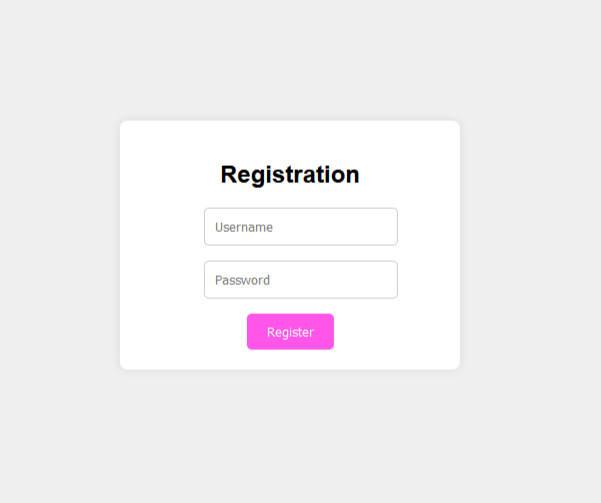
\includegraphics[width=0.7\linewidth]{images/clear_reg}
		\caption{Страница регистрации (поля пустые)}
		\label{fig:clearreg}
	\end{figure}
		
	\begin{figure}[H]
		\centering
		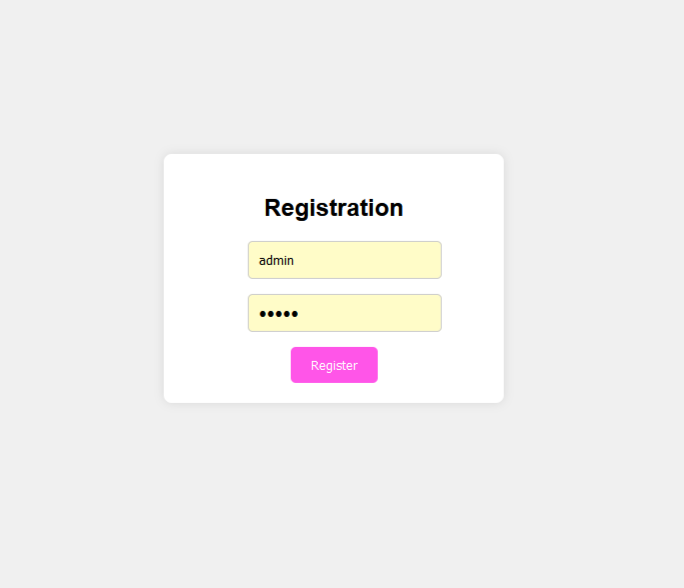
\includegraphics[width=0.7\linewidth]{images/full_reg}
		\caption{Страница регистрации (заполненные поля admin admin)}
		\label{fig:fullreg}
	\end{figure}
	
	\begin{figure}[H]
		\centering
		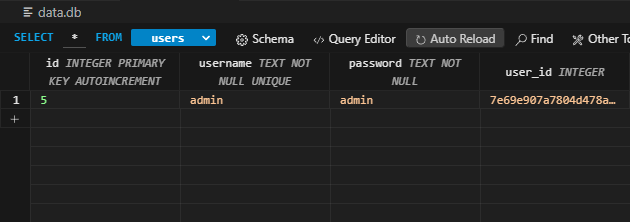
\includegraphics[width=0.7\linewidth]{images/db_admin}
		\caption{База данных после регистрации}
		\label{fig:dbadmin}
	\end{figure}
	
	\item Случай использования: логин пользователя
	\begin{itemize}
		\item Предусловие: пользователь не авторизован в системе, веб-мессенджер доступен по адресу.
		\item Тестовый случай: пользователь переходит по URL ссылке с припиской /login.
		\item Ожидаемый результат: открывается страница логина с полями для ввода логина и пароля (после успешного логина пользователя перекидывает на страницу с мессенджером).
		\item Результаты представлены на рисунках \ref{fig:clearlog} и \ref{fig:fulllog}.
	\end{itemize}
	
	\begin{figure}
		\centering
		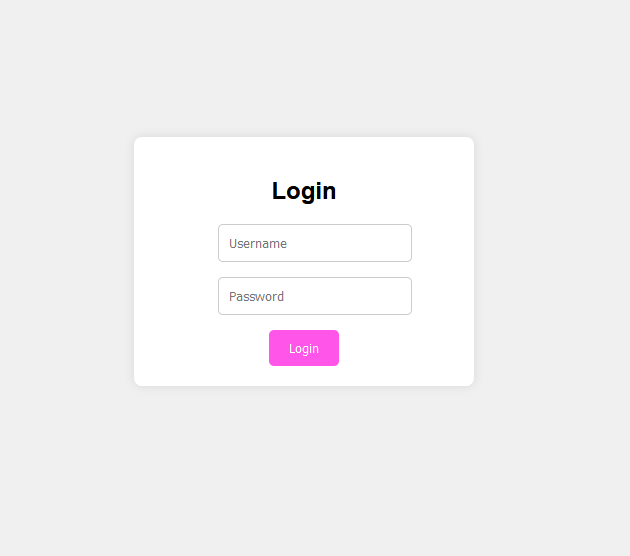
\includegraphics[width=0.7\linewidth]{images/clear_log}
		\caption{Страница логина (поля пустые)}
		\label{fig:clearlog}
	\end{figure}
	
	\begin{figure}
		\centering
		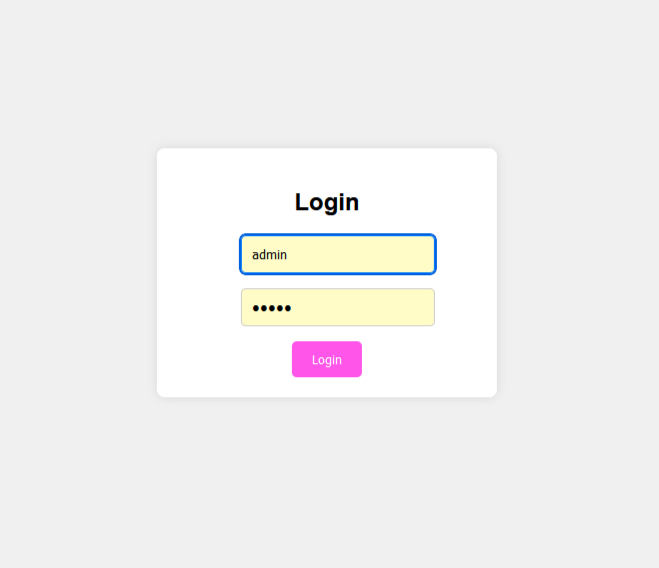
\includegraphics[width=0.7\linewidth]{images/full_log}
		\caption{Страница логина(заполненные поля admin admin)}
		\label{fig:fulllog}
	\end{figure}
		
		
	\item Случай использования: отправка сообщения (без логина)
	\begin{itemize}
		\item Предусловие: пользователь не авторизован в системе.
		\item Тестовый случай: пользователь вводит текст сообщения и нажимает кнопку "Отправить".
		\item Ожидаемый результат: сообщение отправляется, отображаемое имя Guest.
		\item Результаты представлены на рисунках \ref{fig:nonlogguestmes} и \ref{fig:dbuserclear}.
	\end{itemize}
	
	\begin{figure}[H]
		\centering
		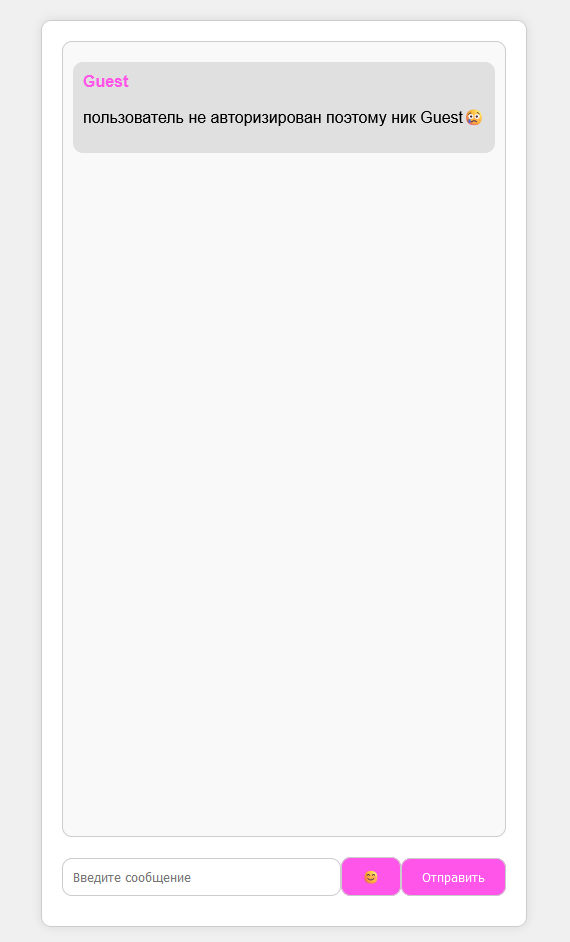
\includegraphics[width=0.7\linewidth]{images/nonlog_guest_mes}
		\caption{Пользователь не вошел и отправил сообщение}
		\label{fig:nonlogguestmes}
	\end{figure}
	
	\begin{figure}[H]
		\centering
		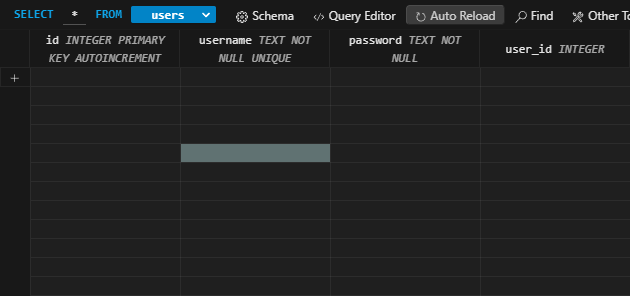
\includegraphics[width=0.7\linewidth]{images/dbuser_clear}
		\caption{Пустая база данных (зарегистрированные пользователи отсутсвуют)}
		\label{fig:dbuserclear}
	\end{figure}
	
		\item Случай использования: отправка сообщения (логин cubemalevich)
	\begin{itemize}
		\item Предусловие: пользователь авторизован в системе.
		\item Тестовый случай: пользователь вводит текст сообщения и нажимает кнопку "Отправить".
		\item Ожидаемый результат: сообщение отправляется, отображаемое имя cubemalevich.
		\item Результаты представлены на рисунках \ref{fig:logcubmes} и \ref{fig:dbmessages}.
	\end{itemize}
	
	\begin{figure}[H]
		\centering
		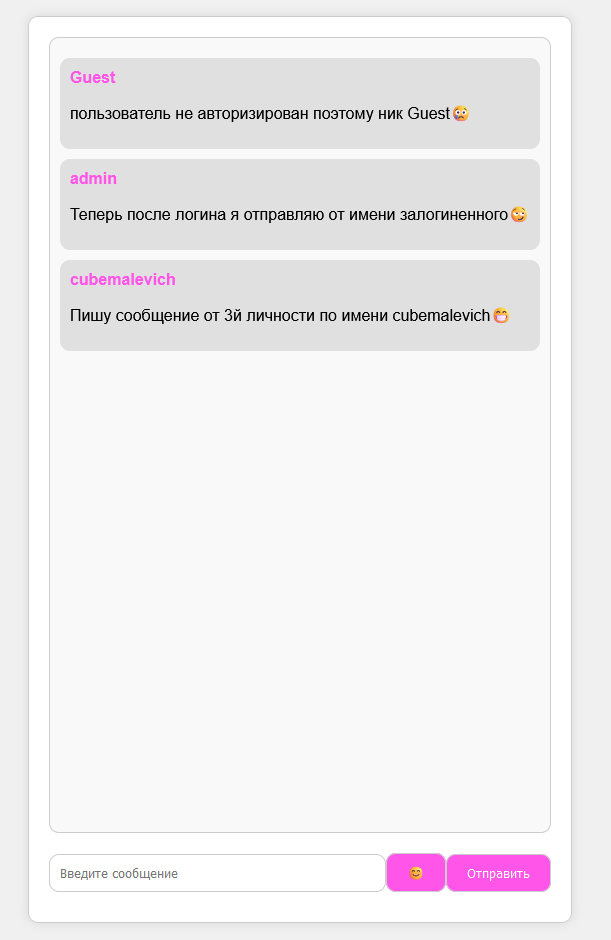
\includegraphics[width=0.7\linewidth]{images/log_cub_mes}
		\caption{Пользователь cubemalevich отправил сообщение}
		\label{fig:logcubmes}
	\end{figure}

	\begin{figure}[H]
		\centering
		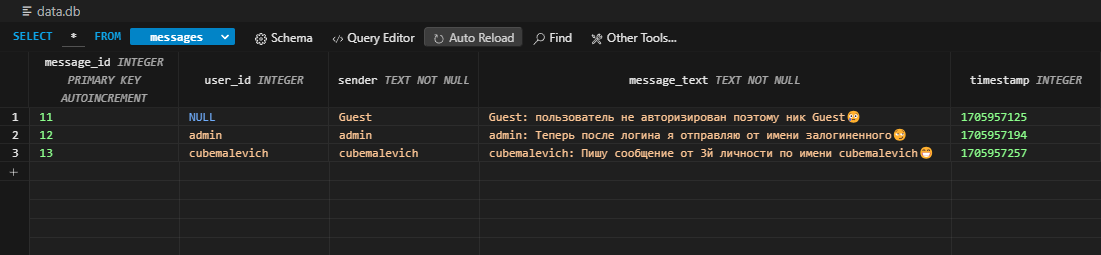
\includegraphics[width=0.7\linewidth]{images/db_messages}
		\caption{База данных с сообщениями}
		\label{fig:dbmessages}
	\end{figure}
	
	\item Случай использования: отправка смайликов
	\begin{itemize}
		\item Предусловие: пользователь авторизован в системе.
		\item Тестовый случай: пользователь нажимает кнопку отправки смайликов.
		\item Ожидаемый результат: открывается "пикер" смайликов, пользователь выбирает смайлик и отправляет.
		\item Результаты представлены на рисунках \ref{fig:smilepicker}, \ref{fig:sendsmile} и \ref{fig:dbmessagessmile}.
	\end{itemize}
	
	\begin{figure}[H]
		\centering
		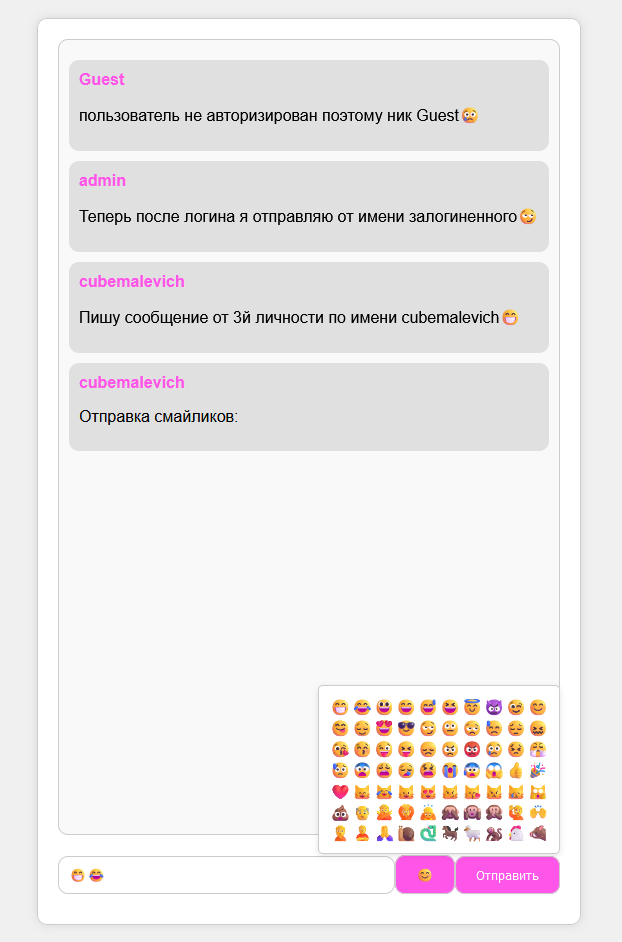
\includegraphics[width=0.7\linewidth]{images/smile_picker}
		\caption{Пикер смайликов}
		\label{fig:smilepicker}
	\end{figure}
		
	\begin{figure}[H]
		\centering
		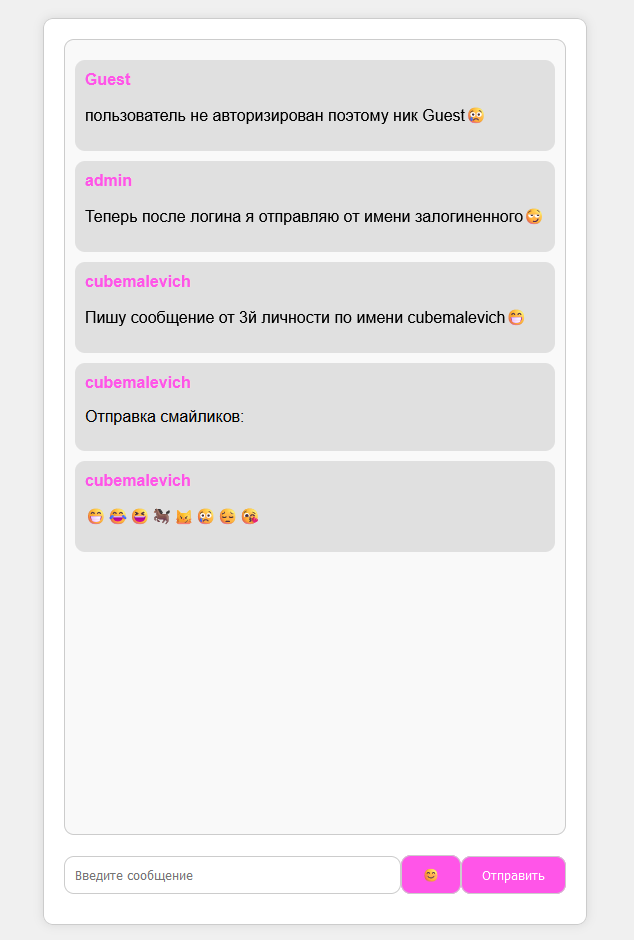
\includegraphics[width=0.7\linewidth]{images/send_smile}
		\caption{Отправленные смайлики}
		\label{fig:sendsmile}
	\end{figure}
	
	\begin{figure}[H]
		\centering
		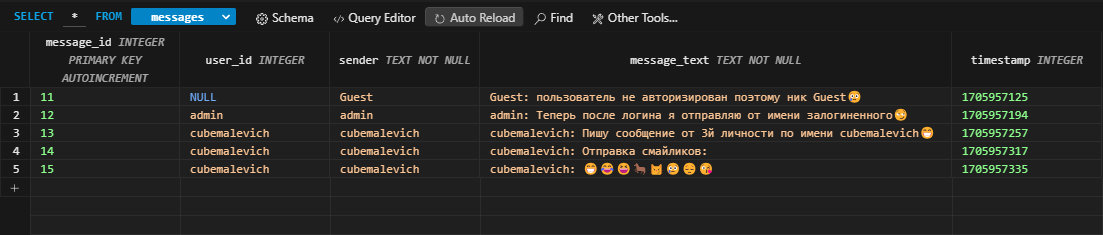
\includegraphics[width=0.7\linewidth]{images/db_messages_smile}
		\caption{База данных с сообщениями}
		\label{fig:dbmessagessmile}
	\end{figure}


\end{enumerate}
